\chapter{Datasets and running conditions}
\label{chap:prod:data}

The data used for this measurement were collected at the very beginning of 
\runtwo\ of the \ac{LHC}, during a special 15-day `early measurements' period.
The number of bunches in the accelerator was gradually increased from 50 to 482 
bunches at the end of the period, with the number colliding at IP8 increasing 
from 36 to 397 bunches.
In addition, the minimum bunch spacing was set to \SI{50}{\nano\second}, as in 
\runone, rather than the nominal \runtwo spacing of \SI{25}{\nano\second}.
These steps were taken primarily for machine safety, as the \ac{LHC} began 
operating at a new centre-of-mass energy, \sqrtseq{13}, never before seen at a 
particle collider.

The machine suffered several technical problems during this period, and so a 
significant amount of time allocated for `physics running' was lost to 
recovery.
At \lhcb, each \ac{LHC} fill is indexed with a number, and this measurement 
uses fills 3976, 3981, 3988, 3992, and 3996.
The combination of these fills corresponds to around \SI{32}{\hour} of 
collisions.
Other fills taken during the early measurements period were excluded from the 
analysis due to them either having short times, usually corresponding to 
unstable beams unfit for physics, or because one or more sub-detector was found 
to be operating incorrectly during data-taking.

The combined dataset used for the measurement corresponds to an integrated 
luminosity, defined in \cref{eqn:prod:introduction:integrated_lumi}, of
\begin{equation}
  \intlumi = \SI{\xsectotlumi}{\per\pico\barn}.
  \label{eqn:prod:xsectotlumi}
\end{equation}
For reference, the total integrated luminosity collected in \runone\ at \lhcb\ 
was \SI{3}{\per\femto\barn}, 600 times more, whilst that for the \sqrtseq{7}\ 
\lhcb\ open charm production measurement was \SI{15}{\per\nano\barn}, 300 times 
less.
All data were taken with \lhcb\ dipole magnet in the `down' polarity, and were 
processed via the Turbo stream data flow, as described in 
\cref{chap:intro:lhcb:detector}.
The selection of events and charm candidates, both in the trigger and offline, 
will be described in \cref{chap:prod:sel}.
A description of the luminosity measurement will now be given.

\section{Luminosity determination}
\label{chap:prod:data:lumi}

The luminosity was measured in a dedicated analysis as part of the general 
\lhcb\ early measurements campaign.
The luminosity is used as input not only for the open charm production analysis 
discussed here, but also in the measurements of \PJpsi and \PB hadron 
production~\cite{LHCb-PAPER-2015-037,LHCb-PAPER-2016-031}, which were also part 
of that campaign.

The instantaneous luminosity is defined in \cref{eqn:intro:lhc:inst_lumi}, and 
can be re-formulated more succinctly as
\begin{equation}
  \lumi = N_{\text{p}}^{2}\revfreq\Omega,
  \label{eqn:prod:data:lumi}
\end{equation}
where $\Omega$ encapsulates the overlapping bunch densities.
If each bunch, 1 and 2, has particle density distributions $\rho_{1}(x, y, z, 
t)$ and $\rho_{2}(x, y, z, t)$, the overlap can be expressed as
\begin{equation}
  \Omega \propto \int \rho_{1}(x, y, z, t)\rho_{2}(x, y, z, t)
                      \dif{x}\dif{y}\dif{z}\dif{t}.
  \label{eqn:prod:data:lumi:profile}
\end{equation}
At \lhcb, two methods have been used to measure the bunch 
profiles~\cite{LHCb-PAPER-2014-047}.
% TODO ok, but what is done with the scan data?
The first is the \ac{VDM} scan, where the beams are scanned across each other 
in fine $x$ and $y$ steps to measure the transverse profile, which is also used 
in the \atlas, \cms, and \alice\ experiments.
It assumes that the profiles in $x$ and $y$ are factorisable, such as being two 
independent Gaussian distributions.
The high precision of the \lhcb\ \velo\ sub-detector allows for the second 
method: the \ac{BGI}.
This method uses gas injected into the \ac{LHC} vacuum inside the \velo\ 
sub-detector to create `beam-gas' interactions.
The vertices of these interactions can be reconstructed using track segments 
formed in the \velo, shown in \cref{fig:prod:data:lumi:bgi_fits}, and the 
distribution of vertices gives the three-dimensional beam profile.

As the \ac{VDM} and \ac{BGI} methods are independent, they serve as 
cross-checks of one another and can be combined in an average if they are 
compatible.
They were both used in an analysis to measure the \runone\ integrated 
luminosity, where a relative uncertainty on the combination of 
\SI{1.16}{\percent} was achieved, the highest precision on a luminosity 
measurement at an \ac{LHC} experiment~\cite{LHCb-PAPER-2014-047}.
For the early measurements campaign, only the data for the \ac{BGI} measurement 
was available, and a precision of \SI{3.8}{\percent} was reached.

Both the \ac{VDM} and the \ac{BGI} methods require special \ac{LHC} running 
conditions.
The data for the luminosity analysis is collected during dedicated fills, the 
data from which is not used for physics analyses.
The absolute luminosity is then determined only for these fills, and so it is 
necessary to translate this to a luminosity measurement for the fills used for 
physics data.
This is done by choosing a set of processes whose rates are proportional to the 
visible \pp\ interaction rate, and using the constant of proportionality as 
measured during the absolute luminosity measurement.
These `luminosity counters', such as the number of tracks reconstructed in the 
\velo, the energy deposited in the hadronic calorimeter, or even the fraction 
of beam-beam crossings where no activity was seen in the detector, are stored 
alongside the data during physics running.
The total luminosity for a dataset used in an analysis is then determined by 
integrating the values from a counter and dividing it by the corresponding 
absolute luminosity calibration constant.

\begin{figure}
  \centering
  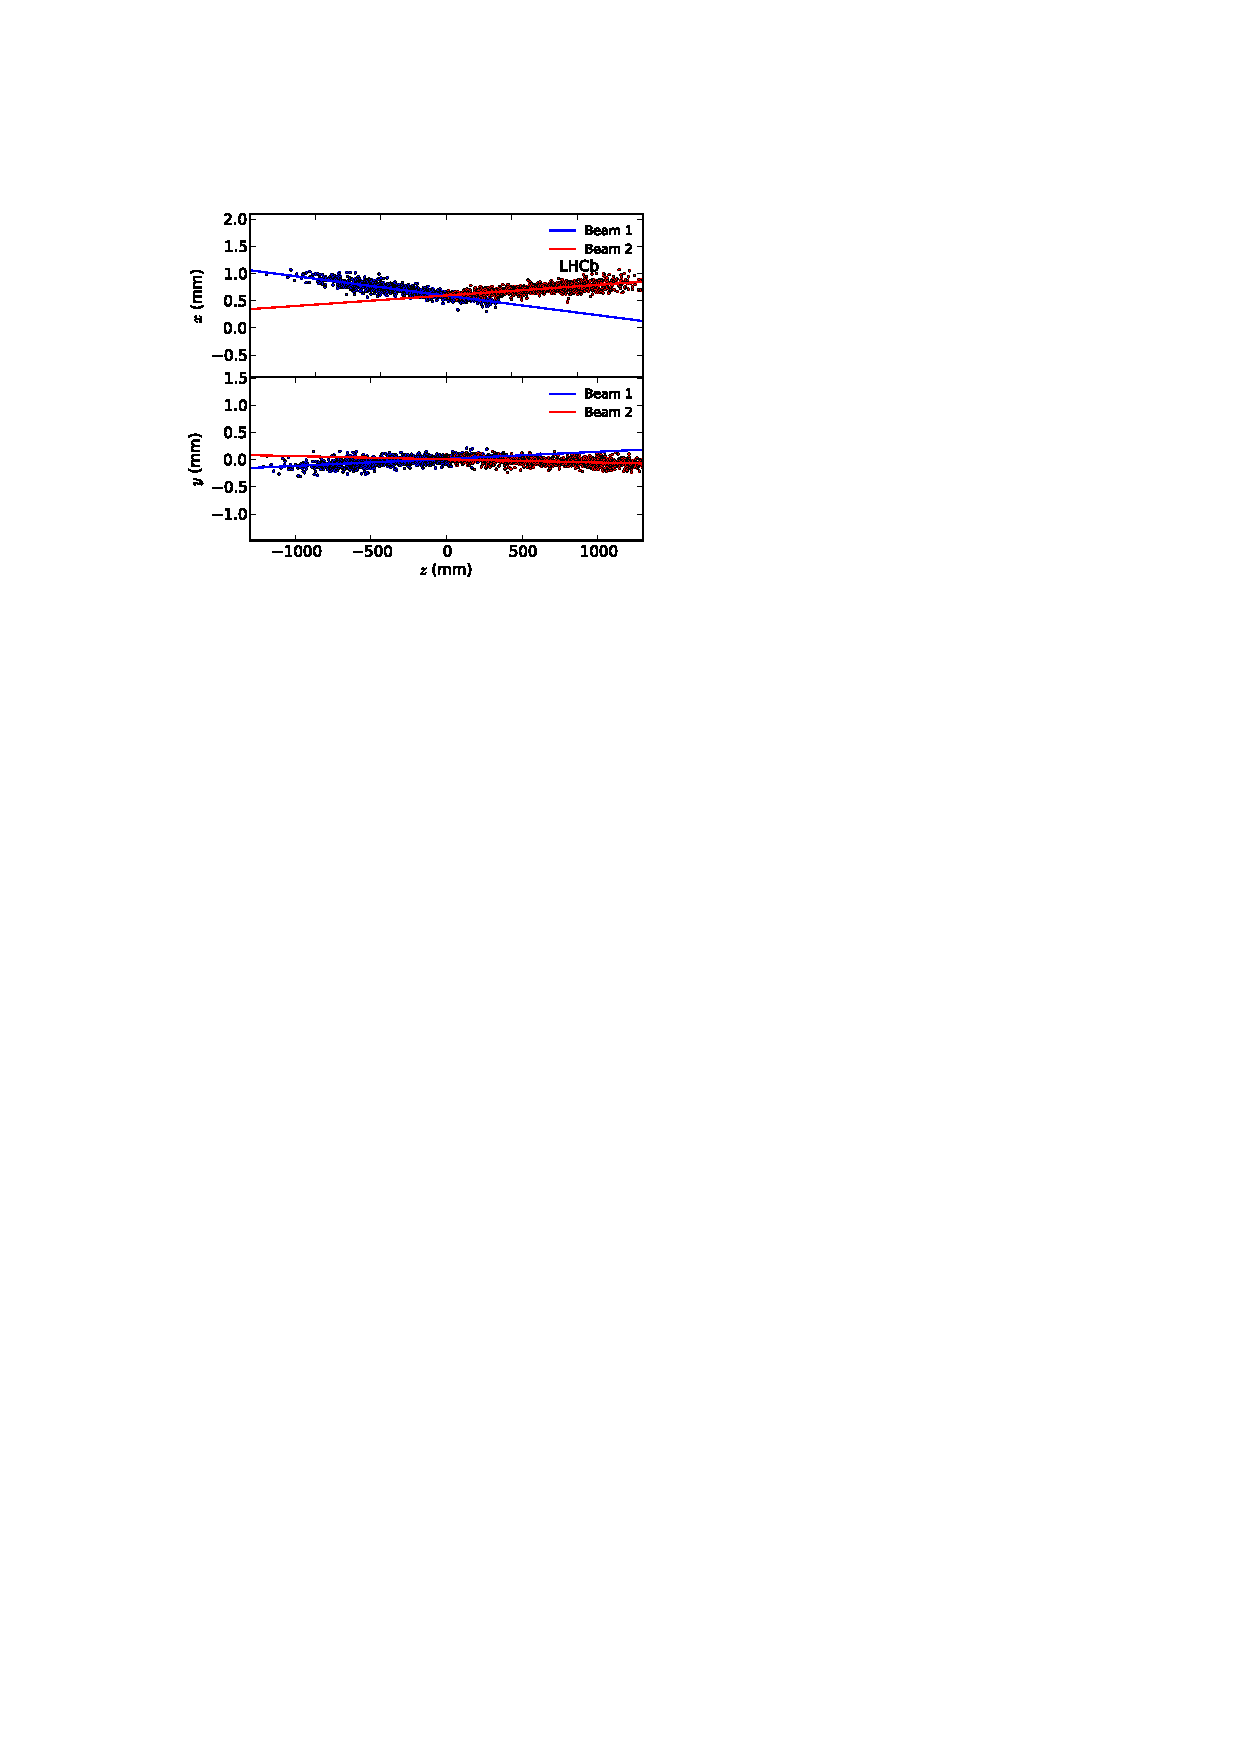
\includegraphics[width=\textwidth]{figures/production/bgi_fits}
  \caption{%
    Projections of fits to beam-gas interaction vertices used as part of a 
    \acl{BGI} luminosity measurement~\cite{LHCb-PAPER-2014-047}.
    The data shown were used for the \ac{BGI} measurement at \sqrtseq{8} in 
    2012.
    For illustrative purposes only the first \num{1000} interaction vertices 
    are shown per beam.
  }
  \label{fig:prod:data:lumi:bgi_fits}
\end{figure}

\section{Simulated data samples}
\label{chap:prod:data:mc}

% TODO describe MC datasets. will need to say this section will appear in the
% Chapter introduction
